\section{Software Testing}
\begin{itemize}
	\item What is Software Testing?
	\begin{itemize}
		\item Running a program in order to find faults
		\begin{itemize}
			\item Examining the code without execution is \underline{not} testing
		\end{itemize}
		\item The main practical approach to validate/verify software
		\begin{itemize}
			\item Formal methods that aim at proving the correctness of a program are not
			scalable
		\end{itemize}
		\item “Program testing can be used to show the presence of bugs, but never to show their absence!” -- Edsger W. Dijkstra
	\end{itemize}
	\item Testing Levels
	\begin{itemize}
		\item Acceptance testing
		\begin{itemize}
			\item Test whether the software is acceptable to the user
		\end{itemize}
		\item System testing
		\begin{itemize}
			\item Test the overall functionality of the system
		\end{itemize}
		\item Integration testing
		\begin{itemize}
			\item Test how modules interact with each other
		\end{itemize}
		\item Module testing
		\begin{itemize}
			\item A module is a collection of related units the are assembled in a file, package, or class
			\item Test modules in isolation including how the components interact with each other
			\item \underline{Responsibility of the programmer}
		\end{itemize}
		\item Unit testing
		\begin{itemize}
			\item Test units (methods individually)
			\item \underline{Responsibility of the programmer}
		\end{itemize}
	\end{itemize}

	\item Black-Box and White-Box Testing
	\begin{itemize}
		\item Black-Box Testing
		\begin{itemize}
			\item Test are derived from external descriptions of the software
		\end{itemize}
		\item White-Box Testing
		\begin{itemize}
			\item Test are derived from source code internals of the software
			\item More expensive to apply
		\end{itemize}
	\end{itemize}

	\item Why is Software Testing Hard?
	\begin{itemize}
		\item Exhaustive testing is infeasible
		\begin{itemize}
			\item e.g. Exhaustively testing a method with two integer parameters would
			require $ \sim \negmedspace 10^{19} $ tests
		\end{itemize}
		\item Random/statistical testing is not effective
	\end{itemize}

	\item Why Do We Test Software?
	\begin{itemize}
		\item Software is everywhere
		\begin{itemize}
			\item Communication, transportation, healthcare, finance, education, etc.
		\end{itemize}
		\item Software failures could have severe consequences
		\begin{itemize}
			\item A 2002 NIST report estimated that defective software costs the U.S. economy \$59.5 billion per year and that improvements in testing could reduce this cost by about a third
			\item In certain areas such as healthcare and transportation, software failures could cost lives
		\end{itemize}
	\end{itemize}

	\item Infamous Software Failures
	\begin{itemize}
		\item Northeast blackout of 2003
		\begin{itemize}
			\item Caused by a failure of the alarm system
			\item Affected 40 million people in USA and 10 million people in Canada
			\item Contributed to at least 11 deaths
			\item Cost around \$6 billion
		\end{itemize}
		\item Ariane 5 explosion (1996)
		\begin{itemize}
			\item Unhandled floating point conversion exception
			\item Estimated loss: \$370 million
		\end{itemize}
		\item NASA’s Mars lander (1999)
		\begin{itemize}
			\item Crashed due to an integration fault
			\item Estimated loss: \$165 million
		\end{itemize}
		\item Boeing 737 Max
		\begin{itemize}
			\item Crashed due to overly aggressive software flight overrides
		\end{itemize}
		\item Boeing A220
		\begin{itemize}
			\item Engines failed after software update allowed excessive vibrations
		\end{itemize}
		\item Toyota brakes failure
		\begin{itemize}
			\item Dozens dead
			\item Thousands of crashes
		\end{itemize}
		\item Therac-25 radiation therapy machine
		\begin{itemize}
			\item Three patients were killed
		\end{itemize}
	\end{itemize}

	\item Fault/Error/Failure
	\begin{itemize}
		\item \textbf{\textit{Software Fault}}: A static defect in the software
		\item \textbf{\textit{Software Error}}: An incorrect internal state that is the manifestation of
		some fault
		\item \textbf{\textit{Software Failure}}: External, incorrect behavior with respect to the requirements or another description of the expected behaviour
		\item The term \textbf{\textit{bug }}is often used informally to refer to all three of fault, error, and failure
		\begin{itemize}
			\item The first computer bug was an actual bug!
		\end{itemize}
		\item Example\\
		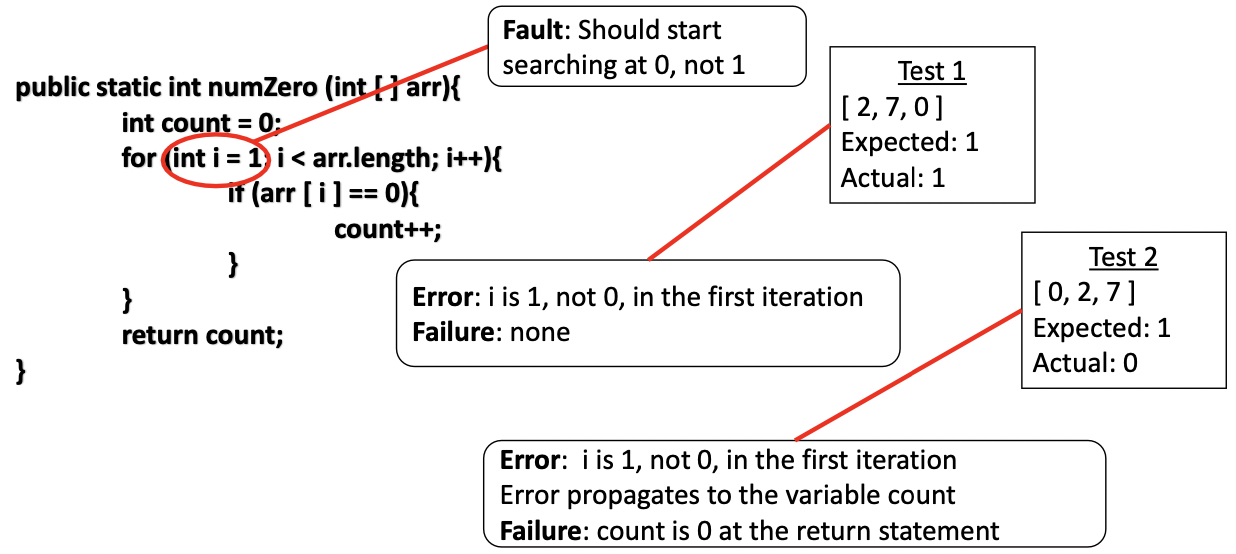
\includegraphics[scale=0.7]{FEF.png}
	\end{itemize}

	\newpage
	\item The RIPR model
	\begin{itemize}
		\item Four conditions are needed for a failure to be observed
		\begin{enumerate}
			\item \textbf{\textit{Reachability}}: a test must reach the location in the program that contains the fault
			\item \textbf{\textit{Infection}}: After the faulty location is executed, the state of the program must be incorrect
			\item \textbf{\textit{Propagation}}: The infected state must propagate through the rest of the execution and cause some output or final state of the program to be incorrect
			\item \textbf{\textit{Revealability}}: The tester must observe part of the incorrect portion of the final program state
		\end{enumerate}
		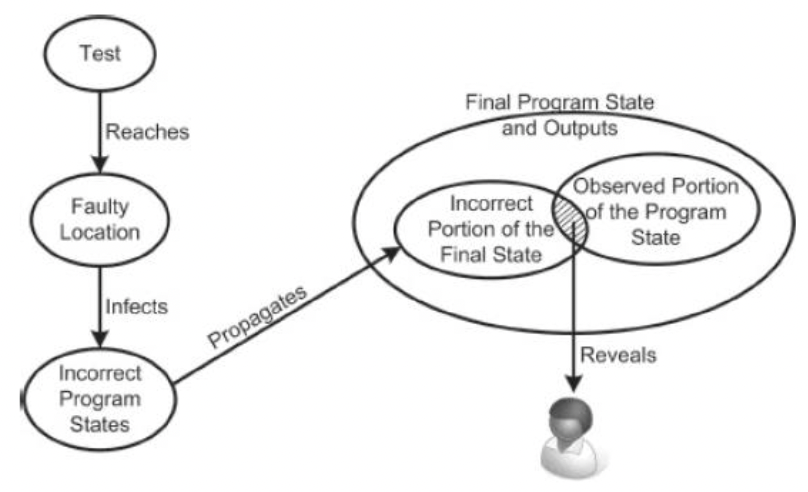
\includegraphics[scale=0.7]{RIPR.png}
	\end{itemize}

	\item Criteria-based Test Design
	\begin{itemize}
		\item \textbf{\textit{Coverage Criterion}}: A rule or collection of rules that impose test requirements on a test set
		\begin{itemize}
			\item e.g. For each statement in the code, there should be at least one test case that covers it
		\end{itemize}
		\item Coverage criteria give us structured, practical ways to search the input space. Satisfying a coverage criterion gives a tester some amount of confidence in two crucial goals:
		\begin{enumerate}
			\item We have looked in many corners of the input space, and
			\item Our tests have a fairly low amount of overlap
		\end{enumerate}
		\item Criteria subsumption
		\begin{itemize}
			\item $ C_1 $ subsumes $ C_2 $ if and only if every test set that satisfies $ C_1 $ satisfies $ C_2 $
		\end{itemize}
	\end{itemize}

	\item Graph Coverage
	\begin{itemize}
		\item The software is modeled as a graph where nodes and edges could represent:
		\begin{itemize}
			\item Methods and calls
			\item Statements and branches
			\item Etc.
		\end{itemize}
		\item Coverage criteria are defined based on the graph. For example:
		\begin{itemize}
			\item Cover every node
			\item Cover every edge
			\item Cover every path
			\item Etc.
		\end{itemize}


		\item Example (Control Flow Graph)\\
		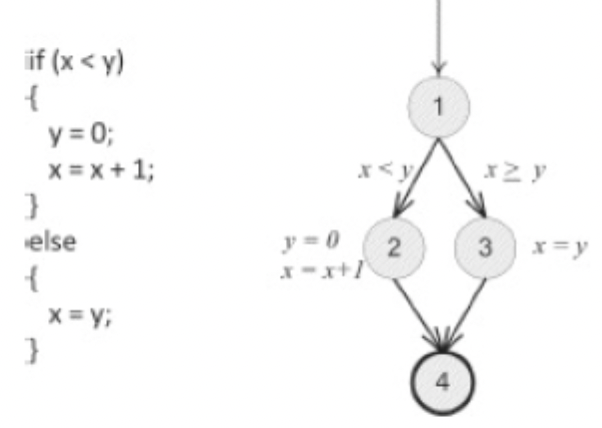
\includegraphics[scale=0.7]{CFG.png}
	\end{itemize}

	\item Logic Coverage
	\begin{itemize}
		\item Involves the boolean expressions of the code
		\item Coverage criteria include:
		\begin{itemize}
			\item Predicate coverage
			\item Clause coverage
			\item Combinational coverage
			\item Etc.
		\end{itemize}
		\item Example
		\begin{Verbatim}
	if(((a>b) || c) && (x<y))
	...
	else
	...
		\end{Verbatim}
		\item Predicate coverage
		\begin{itemize}
			\item The test set should make each predicate evaluate to true and false
			\item e.g. $ ((a>b) \, || \, c) \, \&\& \, (x<y) = \{\text{True}, \text{False}\} $
		\end{itemize}
		\item Clause coverage
		\begin{itemize}
			\item The test set should make each clause evaluate to true and false
			\item e.g. $ (a>b) = \{\text{True}, \text{False}\}, c = \{\text{True}, \text{False}\}, (x<y) = \{\text{True}, \text{False}\} $
		\end{itemize}
	\end{itemize}

	\item Active clause coverage
	\begin{itemize}
		\item Clause coverage has a weakness
		\begin{itemize}
			\item The values do not always make a difference
		\end{itemize}
		\item A clause $ c_i$ in predicate $ p $, called the major clause, determines $ p $ \textit{if and only if} the values of the remaining minor clauses $ c_j $ are such that changing $ c_i $ changes the value of $ p $
		\item Two requirements for each $ c_i $: $ c_i $ evaluates to true and $ c_i $ evaluates to false
		\item This is a form of MCDC, which is required by the FAA for safety critical
		software

	\end{itemize}

	\item Inactive clause coverage
	\begin{itemize}
		\item Ensures that “major” clauses do not affect the predicates
		\item Four requirements for each $ c_i $
		\begin{enumerate}
			\item $c_i$ evaluates to true with p true
			\item $c_i$ evaluates to false with p true
			\item $c_i$ evaluates to true with p false
			\item $c_i$ evaluates to false with p false
		\end{enumerate}
		\item Example
		\begin{itemize}
			\item Testing the control software for a shutdown system in a reactor where the specification states that the status of a particular valve (\textbf{open} vs. \textbf{closed}) is relevant to the reset operation in \textbf{Normal} mode, but not in \textbf{Override} mode
		\end{itemize}
	\end{itemize}

	\item Test Oracles
	\begin{itemize}
		\item A \textit{test oracle} is an encoding of the expected results of a given test
		\begin{itemize}
			\item e.g. JUnit assertion
		\end{itemize}
		\item Must strike a balance between checking too much (unnecessary cost) and checking too little (perhaps not revealing failures)
		\item What should be checked?
		\begin{itemize}
			\item The output state is everything that is produced by the software under test, including outputs to the screen, file, databases, messages, and signals
			\item Each test should have a goal and testers should check the output(s) that are mainly related to that goal
			\begin{itemize}
				\item At the unit testing level, checking the return values of the methods and returned parameter values are almost always enough
				\item At the system level, it is usually sufficient to check the directly visible output such as to the screen
			\end{itemize}
		\end{itemize}

		\item How to determine what the correct results are
		\begin{itemize}
			\item Specification-Based direct verification of outputs
			\begin{itemize}
				\item e.g. “a \textbf{sort} program should produce a permutation of its input in increasing order ”
				\item Specifications are hard to write
			\end{itemize}
			\item Redundant computations
			\begin{itemize}
				\item Refer to another trustworthy implementation of the program
				\item Usually used for regression testing
			\end{itemize}
			\item Consistency checks
			\begin{itemize}
				\item Check whether certain properties hold (e.g. a value representing probability
				should neither be negative nor larger than one)
			\end{itemize}
		\end{itemize}
	\end{itemize}
\end{itemize}
